\documentclass[12pt]{article}

\usepackage{amsmath}
\usepackage{array}
\usepackage{caption}
\usepackage[top=1in, bottom=1in, left=0.75in, right=0.75in]{geometry}
\usepackage{graphicx}
\usepackage[colorlinks=true, allcolors=blue]{hyperref}
\usepackage[utf8]{inputenc}
\usepackage{multirow}
\usepackage{pdfpages}
\usepackage[section]{placeins}

\graphicspath{{figures/}}

\begin{document}

\begin{titlepage}
  \begin{center} \LARGE
    \vspace*{1.5in}

    ECE 272 Pre-Lab 5

    Fall 2018

    \vfill

    Serial Peripheral Interface (SPI)

    Phi Luu

    \vfill

    October 31\textsuperscript{st}, 2018

    Grading TA: Edgar Perez

    \vspace{1.5in}
  \end{center}
\end{titlepage}

\begin{enumerate}
  \item Simulate lab 4 in Modelsim.

  In lab 4, I compiled and simulated the project on ModelSim and obtained the following waveforms:

  \begin{figure}[ht]
    \centering
    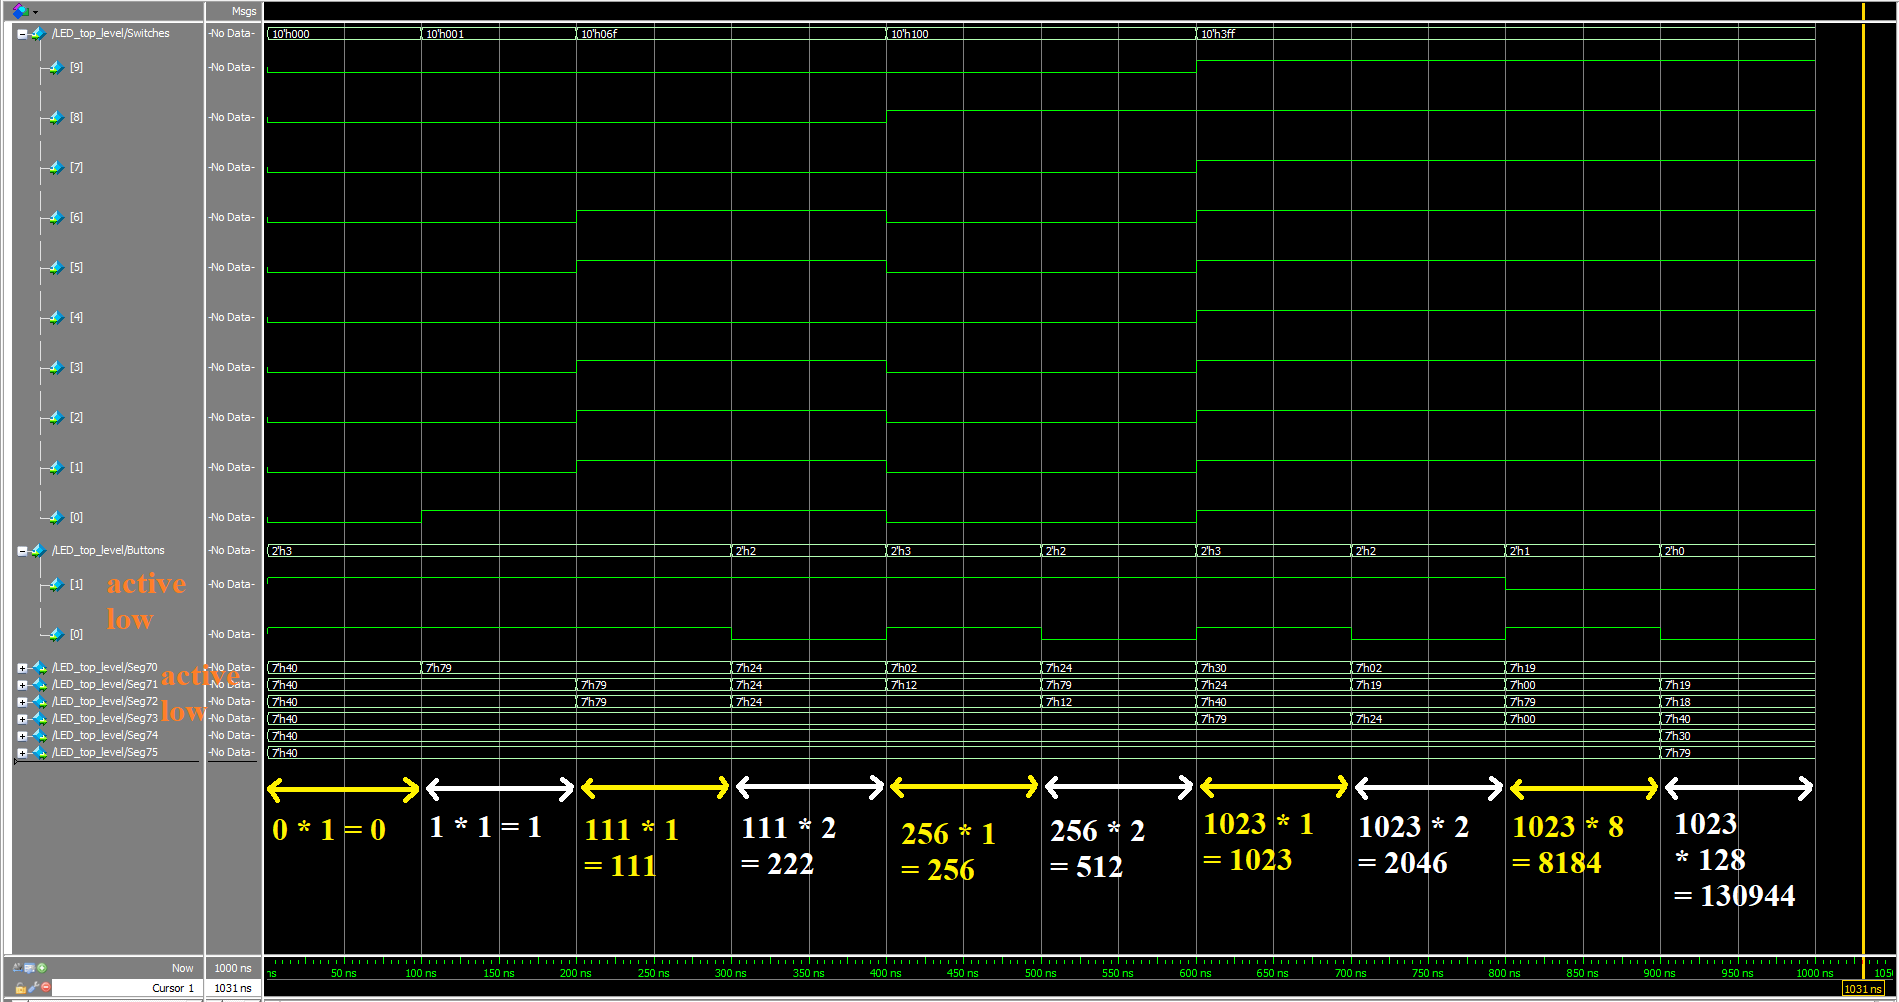
\includegraphics[width=\textwidth]{lab4_simulation.png}
    \caption{Simulation waveform of a few test examples. \href{https://i.imgur.com/1UjCN6E.png}{High-resolution image}}
    \label{figure:3}
  \end{figure}

  Each 100-ns interval (2 columns) is a test case. Each of the test cases' inputs and output are specified with a two-way arrow. For example, from 100 ns to 200 ns (from the third column to the fourth column), the switch input is equivalent to a $1$ in decimal system (\textit{SW1} turned on and all other switches turned off), and the button input is equivalent to a $1$ in decimal system (all buttons not pressed), and the output of all 6 seven-segment displays is $000001$ (reading from $\text{Seg75}$ to $\text{Seg70}$).

  Using the same way to read the waveforms, I obtained the results of all example test cases. Since the results were consistent with mathematical calculations, it is strongly suggestive that the simulation of the project was a success and that the program was implemented correctly.

\end{enumerate}

\end{document}
